\documentclass[journal, onecolumn]{IEEEtran}
\IEEEoverridecommandlockouts
% The preceding line is only needed to identify funding in the first footnote. If that is unneeded, please comment it out.
\usepackage{cite}
\usepackage{amsmath,amssymb,amsfonts}
\usepackage{algorithmic}
\usepackage{textcomp}
\usepackage{theorem,caption,extarrows,mathrsfs}
\usepackage{graphicx,xcolor,hyperref,booktabs,float,subfig,overpic}
\usepackage{tikz}
\usepackage[european]{circuitikz}
\usetikzlibrary{calc}
\usepackage{pgfplots,grffile}
\usepackage{fontspec}
\usepackage[skins]{tcolorbox}
\setmainfont{STIX Two Text}
\setsansfont{CMU Sans Serif}
\setmonofont{Sarasa Fixed SC Nerd Font}
\pgfplotsset{compat=newest}
%% the following commands are needed for some matlab2tikz features
\usetikzlibrary{plotmarks}
\usetikzlibrary{arrows.meta}
\usetikzlibrary{calc}
\usepgfplotslibrary{patchplots}
\def\BibTeX{{\rm B\kern-.05em{\sc i\kern-.025em b}\kern-.08em
T\kern-.1667em\lower.7ex\hbox{E}\kern-.125emX}}
%% href setup
\usepackage[normalem]{ulem}
\definecolor{mylinkcolor}{HTML}{0078D4}
\definecolor{myulcolor}{HTML}{00487F}
\hypersetup{
	hidelinks=true
}
% \newcommand\reduline{\bgroup\markoverwith{\textcolor{red}{\rule[-0.5ex]{2pt}{0.4pt}}}\ULon}
\makeatletter
  \newcommand\reduline{\bgroup\markoverwith{\textcolor{red}{\rule[-0.5ex]{2pt}{0.4pt}}}\ULon}
  \UL@protected\def\bluedotuline{\leavevmode \bgroup
    \UL@setULdepth
    \ifx\UL@on\UL@onin \advance\ULdepth2\p@\fi
    \markoverwith{\begingroup
       %\advance\ULdepth0.08ex
       \lower\ULdepth\hbox{\kern.06em \textcolor{myulcolor}{.}\kern.04em}%
       \endgroup}%
    \ULon}
  \UL@protected\def\bluedashuline{\leavevmode \bgroup
    \UL@setULdepth
    \ifx\UL@on\UL@onin \advance\ULdepth2\p@\fi
    \markoverwith{\kern.13em
    \vtop{\color{myulcolor}\kern\ULdepth \hrule width .3em}%
    \kern.13em}\ULon}
\makeatother

\newcommand{\myhy}[1]{%
	\hyperref[#1]{\color{mylinkcolor}\bluedotuline{\textit{\ttfamily\footnotesize #1}}}%
}
%% Listings setup
\usepackage{listings}
\lstset{
    basicstyle          =   \sffamily,          % 基本代码风格
    keywordstyle        =   \bfseries,          % 关键字风格
    commentstyle        =   \rmfamily\itshape,  % 注释的风格,斜体
    stringstyle         =   \ttfamily,  % 字符串风格
    flexiblecolumns,                % 别问为什么,加上这个
    numbers             =   left,   % 行号的位置在左边
    showspaces          =   false,  % 是否显示空格,显示了有点乱,所以不现实了
    numberstyle         =   \tiny\ttfamily,    % 行号的样式,小五号,tt等宽字体
    showstringspaces    =   false,
    captionpos          =   t,      % 这段代码的名字所呈现的位置,t指的是top上面
    frame               =   shadowbox,   % 显示边框
    rulesepcolor=\color{red!20!green!20!blue!20}
}

\lstdefinestyle{Python}{
    language        =   Python, % 语言选Python
    backgroundcolor=\color{backpycol},
    basicstyle      =   \ttfamily,
    numberstyle     =   \ttfamily,
    keywordstyle    =   \color{blue},
    keywordstyle    =   [2] \color{teal},
    stringstyle     =   \color{magenta},
    commentstyle    =   \color[HTML]{338AAF}\ttfamily,
    breaklines      =   true,   % 自动换行,建议不要写太长的行
    columns         =   fixed,  % 如果不加这一句,字间距就不固定,很丑,必须加
    basewidth       =   0.5em,
}
\definecolor{codegreen}{rgb}{0,0.6,0}
\definecolor{codegray}{rgb}{0.5,0.5,0.5}
\definecolor{codepurple}{rgb}{0.58,0,0.82}
\definecolor{backcolour}{rgb}{0.95,0.95,0.92}
\definecolor{backpycol}{rgb}{0.97,0.95,0.97}
\lstdefinestyle{C++}{
    language =[ANSI]C,
    backgroundcolor=\color{backcolour},
    commentstyle=\color[HTML]{338AAF}\ttfamily,
    keywordstyle=\sffamily\bfseries\color{magenta},
    numberstyle=\color{codegray},
    stringstyle=\color{codepurple},
    basicstyle=\ttfamily,
    breakatwhitespace=false,
    breaklines=true,
    basewidth=0.5em,
    captionpos=b,
    columns=fixed,
    frame=shadowbox,
    keepspaces=true,
    numbers=left,
    numbersep=5pt,
    showspaces=false,
    showstringspaces=false,
    showtabs=false,
    tabsize=4
}
\lstdefinestyle{matlab}{
    language=matlab,
    backgroundcolor=\color{backcolour},
    commentstyle=\color[HTML]{338AAF}\ttfamily,
    keywordstyle=\sffamily\bfseries\color{magenta},
    numberstyle=\color{codegray},
    stringstyle=\color{codepurple},
    basicstyle=\ttfamily,
    breakatwhitespace=false,
    breaklines=true,
    basewidth=0.5em,
    captionpos=b,
    columns=fixed,
    keepspaces=true,
    numbers=left,
    numbersep=5pt,
    showspaces=false,
    showstringspaces=false,
    showtabs=false,
    tabsize=4,
    frame=shadowbox
}
\definecolor{mygreen}{rgb}{0,0.6,0}
\definecolor{mygray}{rgb}{0.5,0.5,0.5}
\definecolor{mymauve}{rgb}{0.58,0,0.82}
\definecolor{bggray}{rgb}{0.93,0.95,0.94}
\lstdefinestyle{pseudocode}{
    backgroundcolor=\color{bggray},
    columns=fullflexible,
    tabsize=4,
    breaklines=true,               % automatic line breaking only at whitespace
    captionpos=b,                  % sets the caption-position to bottom
    commentstyle=\color{mygreen},  % comment style
    escapeinside={\%*}{*)},        % if you want to add LaTeX within your code
    keywordstyle=\color{blue},     % keyword style
    stringstyle=\color{mymauve}\ttfamily,  % string literal style
    frame=shadowbox,
    rulesepcolor=\color{red!20!green!20!blue!20},
    % identifierstyle=\color{red},
    language=c++,
    numbers=left,
    numberstyle=\small\color{codegray},
    basicstyle=\ttfamily,% size of fonts used for the code
    escapeinside=``,
    xleftmargin=0.6em,
    xrightmargin=0.6em,
    aboveskip=1em
}
\lstdefinestyle{Fortran}{
    language =fortran,
    backgroundcolor=\color{backcolour},
    commentstyle=\color[HTML]{338AAF}\ttfamily,
    keywordstyle=\sffamily\bfseries\color{magenta},
    numberstyle=\small\color{codegray},
    stringstyle=\color{codepurple},
    basicstyle=\ttfamily,
    breakatwhitespace=false,
    breaklines=true,
    basewidth=0.5em,
    captionpos=b,
    columns=fixed,
    frame=shadowbox,
    keepspaces=true,
    numbers=left,
    numbersep=5pt,
    showspaces=false,
    showstringspaces=false,
    showtabs=false,
    tabsize=4
}

\title{EE332 Lab2: Divide-Conquer Implementation of 16-4 Priority Encoder}
\author{
	\IEEEauthorblockN{1\textsuperscript{st} Qiu Kunyuan}
	\IEEEauthorblockA{
		\textit{EEE. Southern University of Science and Technology}\\
		Shenzhen, PRC\\
		11913019@mail.sustech.edu.cn
	}
}
\begin{document}
\maketitle
% !TEX root=./report_lab2.tex

\begin{abstract}
	This report focuses on the difference between cascaded structure and tree structure in the Verilog implementation of 16-4 priority encoder. The timing optimization of combinational logic circuits with a large number of inputs is carried out by the divide and conquer method, and the pipelining method is also employed. Therefore, the routing results are obtained with satisfactory delays and no race-hazard jitters.

	Code for this experiment can be found at \myhy{https://github.com/KagaJiankui/EE332-2024S/tree/master/lab3/lab3.srcs}.
\end{abstract}
\vspace{1em}
\begin{IEEEkeywords}
	FPGA, programmable logic, priority coder, divide-conquer method, pipelining, -hazard condition, jitter, delay
\end{IEEEkeywords}

\section{Introduction}

There are typically two main implementations of priority encoders in Verilog designs: cascaded architecture and tree architecture.

\begin{itemize}
	\item \textbf{Cascaded architecture}: A cascaded architecture is a serial structure that groups input signals and encodes them within each group, and then these results are cascaded. Such a structure enjoys the simplicity of implementation, but suffers from the disadvantage that the delay increases with the increase in the number of input signals.
	\item \textbf{Tree architecture}: A tree architecture is a parallel structure that encodes all the input signals simultaneously. Benefit of this structure is its speed as all the operations are performed in parallel. However, the demerit of this structure is the requirement of more hardware resources.
\end{itemize}

\subsection{Cascaded Architecture}

The code of cascaded priority encoder is \lstinline{if-else} statements organized along with the order of MSB to LSB. Thus, the cascaded priority encoder can be easily modeled by the following Verilog code with parameter \lstinline{digit}:

\begin{lstlisting}[language=verilog, style=verilog]
module encoder
  #(
    parameter digit=8
    parameter digit_output=3
  )
  (
    input  [digit-1:0] x
    input  en,
    output reg [digit_output-1:0]y
  );
  integer i;
  always @(x or en) begin
    if (en) begin
      y = 0;
      for( i = 0; i <= digit - 1; i = i+1)
          if(x[i] == 1)  y = i[digit-1:0];
    end
    else  y = 0;
  end
endmodule
\end{lstlisting}

For 8-3 encoder, the module is instantialized with parameter \lstinline{.digit(8), .digit_out(3)}(note that the width of input and output bus is designated separately since Verilog, as an HDL, lacks exponential operation even in parameterization) that generates the following if-else statements,

\begin{lstlisting}[language=verilog,style=verilog]
module encoder (
  input [7:0] x,
  input en,
  output reg [2:0] y,
  output reg v
);
  always @ (x or en)
    if (x>0 & en==1) begin
      if (x[7]) y = 3'b111;
      else if (x[6]) y = 3'b110;
      else if (x[5]) y = 3'b101;
      else if (x[4]) y = 3'b100;
      else if (x[3]) y = 3'b011;
      else if (x[2]) y = 3'b010;
      else if (x[1]) y = 3'b001;
      else if (x[0]) y = 3'b000;
      else y = 3'b000;
    end
    else begin
      y = 0;
      v = 0;
  end
endmodule
\end{lstlisting}

and the schematic (\ref{cascaded_83_encoder}) of the elaboration result is basically directly translated from the HDL description, which are cascaded MUXs.

\begin{figure}[htpb]
	\begin{center}
		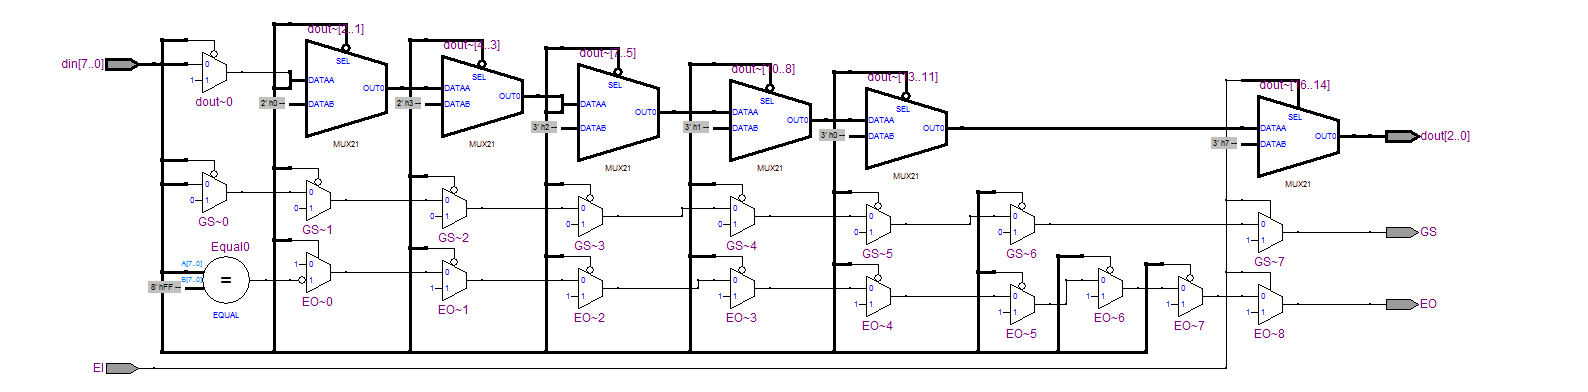
\includegraphics[width=0.98\textwidth]{report_lab3.assets/20240321191356.png}
		\caption{Synthesis result of parameterized 8-3 priority encoder}
		\label{cascaded_83_encoder}
	\end{center}
\end{figure}

For 4-2 encoder, the module is instantialized with parameter \lstinline{.digit(4), .digit_out(2)},

\lstinputlisting[language=verilog, style=verilog]{../../../lab3/lab3.srcs/sources_1/new/encoder4x2_cas.v}

which is elaborated into similiar schematic (\ref{cascaded_42_encoder}):

\begin{figure}[htpb]
	\begin{center}
		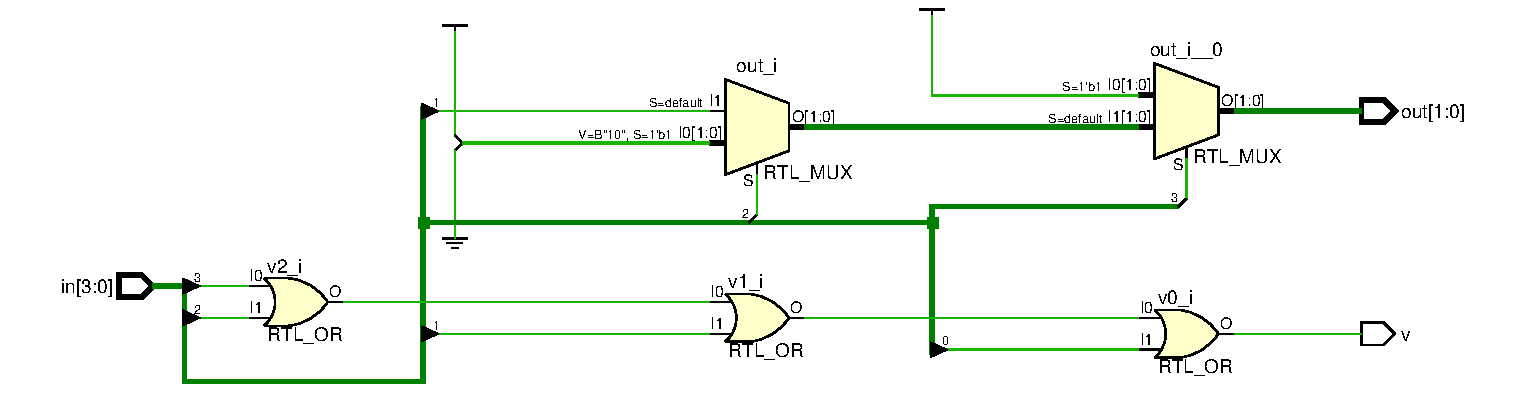
\includegraphics[width=0.80\textwidth]{report_lab3.assets/encoder42_cas_elab_1.pdf}
		\caption{Synthesis result of parameterized 4-2 priority encoder}
		\label{cascaded_42_encoder}
	\end{center}
\end{figure}

\subsection{Tree Architecture}

The encoder organized in tree architecture is a reverse binary tree or quadruple tree, as depicted in left of Fig.(\ref{tree_depict}). The leaf nodes at the bottom level are priority encoders with low input width, while the nodes at higher level are usually MUXs and gates that combines the output from bottom level leaf nodes with their priority.

\begin{figure}[htpb]
	\begin{center}
		\subfloat[Abstraction of Architecture]{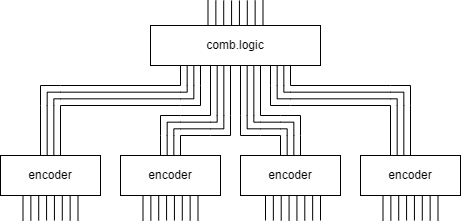
\includegraphics[width=0.45\textwidth]{report_lab3.assets/tree_encoder.png}}\hspace{0.05\columnwidth}
		\subfloat[Combinational Logic Selector]{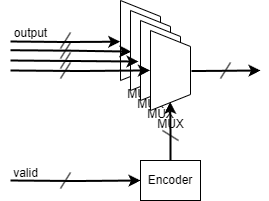
\includegraphics[width=0.45\textwidth]{report_lab3.assets/tree_comb_logic.png}}
		\caption{Architecture Depiction}
		\label{tree_depict}
	\end{center}
\end{figure}

The internal implementation of the combinational logic block is shown in right of Fig.(\ref{tree_depict}). an encoder layer and the adjacent upper combinational logic node, the combinational logic node consists of a set of multiplexers corresponding to the outputs of each bit from each encoder, as well as an encoder generating a line-select signal, with an input width equal to the number of encoders.

In the designs with building block encoder similiar to 74HC148, an encoder IC with \textit{validity} output, the output is therefore composed by the output of the building blocks:

\begin{eqnarray}
	\mathbf{valid}[i]&=&\mathop{\mathrm{OR}}(\mathbf{input}[i])\\
	\mathbf{Q}&=&i*W_{bb}+\mathbf{output}[\mathbf{valid}]
\end{eqnarray}

where the bolded signal name represents bus, the block bracket represents indexing from bus, the variable \(i\) denotes the valid encoder (the location of the highest input bit), and the variable \(W_{bb}\) denotes the input width of the building block encoder.

For a priority encoder with input bitwidth \(W_{input}\), output bitwidth \(W_{output}\), it is obvious that the output bitwidth is the bottom 2 logarithm of the input bitwidth. To employ the tree architecture, the input is splitted the input bitwidth into \(S=W_{input}/W_{bb}\) slices.

\begin{eqnarray}
	W_{output}&=& \log_2 W_{input} \\
	\Rightarrow W_{output}-\log_2 W_{bb} &=& \log_2 \left(\frac{W_{input}}{W_{bb}}\right) \\
	&\Leftrightarrow &
	\begin{cases}
		\log_2 W_{bb}=W_{output}-\log_2 S, \\
		\log_2 S=W_{slice}
	\end{cases}
\end{eqnarray}

Therefore, by converting the multiplication in Eq.(2) into bitwise operations, with respect to the power-2 integrity of S and W, the derivation is clear, that the lower \(W_{bb}\) bits of the output bit is the encoded output of each slice, and the higher \(W_{slice}\) bits is the serial number of the building block encoder with valid state.

For a 16-4 priority encoder in tree architecture, with the building block selected as 4-2 priority encoder with validity indication port, all the parameters can be evaluated from Eq.(5)

\begin{equation}
	W_{output}=\log_2 16=4, S=16/4=4, W_{slice}=2, \log_2 W_{bb}=W_{output}-W_{slice}=2
\end{equation}

Then the verilog modeling is performed intuitively:

\lstinputlisting[language=verilog, style=verilog]{../../../lab3/lab3.srcs/sources_1/new/encoder16x4.v}

which results in the Fig.(\ref{164_elaborated}) after elaboration, and Fig.(\ref{164_synthesis}) after synthesis:

\begin{figure}[htpb]
  \begin{center}
    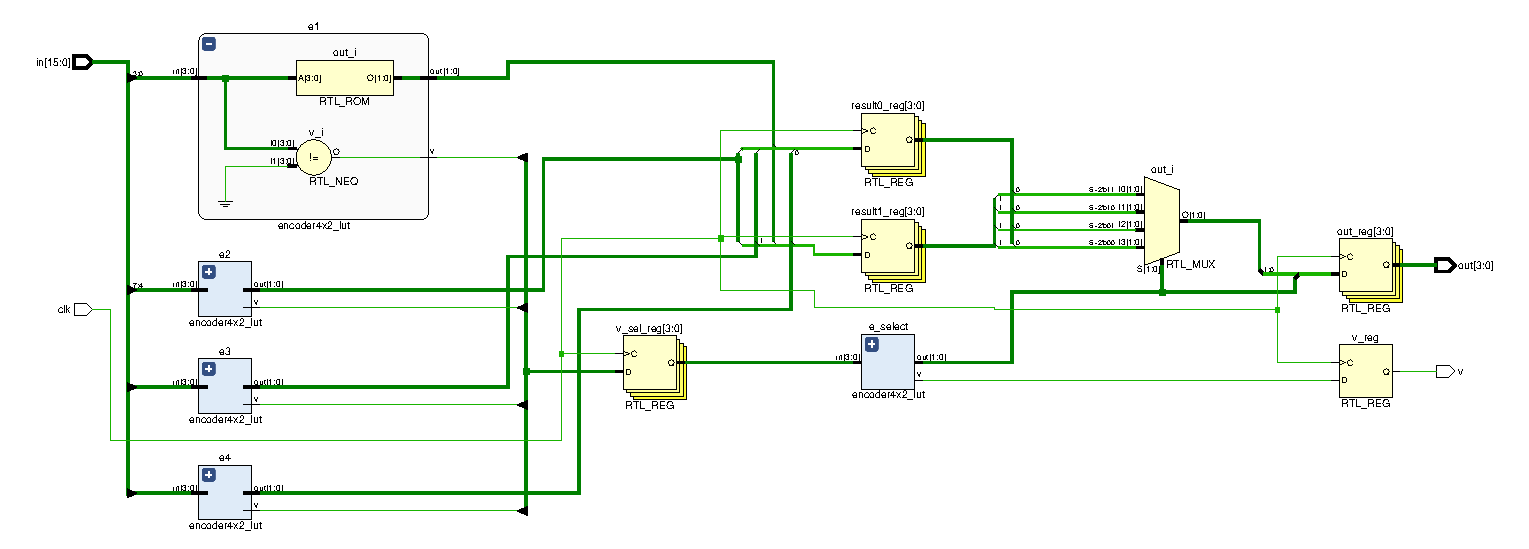
\includegraphics[width=0.80\textwidth]{report_lab3.assets/encoder42_LUT_elab_1.pdf}
    \caption{Elaborated schematic of 16-4 encoder}
    \label{164_elaborated}
  \end{center}
\end{figure}

\begin{figure}[htpb]
  \begin{center}
    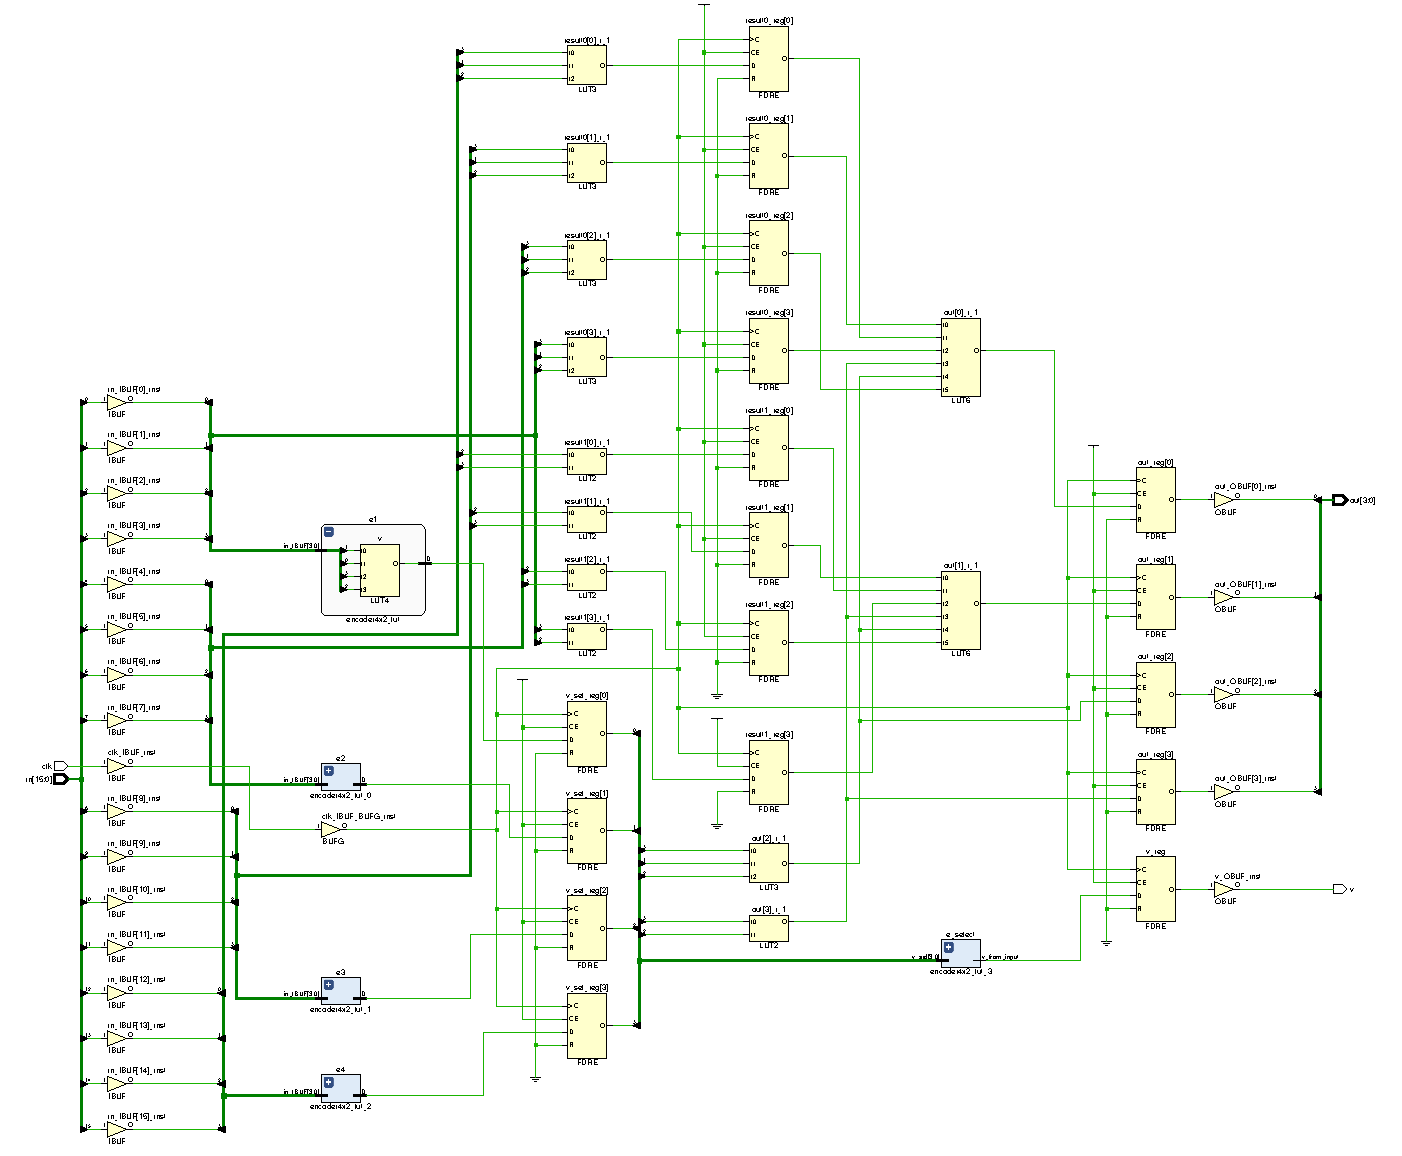
\includegraphics[width=0.80\textwidth]{report_lab3.assets/encoder42_LUT_1.pdf}
    \caption{Synthesized schematic of 16-4 encoder}
    \label{164_synthesis}
  \end{center}
\end{figure}

\section{Time Complexity Discussion and Optimization}

The tree-structured prioritized encoder applies the idea of division and conquering method, which breaks down the big problem into small problems, and then combines the solutions of the small problems into the solution to the big problem. Each layer of the encoder works in parallel, effectively reducing the output delay.

\subsection{Elaboration Stage Analysis}

With the derivation in the section above, it is possible to portrait a model (\ref{data_model}) of the internal data flow in the tree architecture, for the evaluation of the total time complexity (device gate delay):

\begin{figure}[htpb]
  \begin{center}
    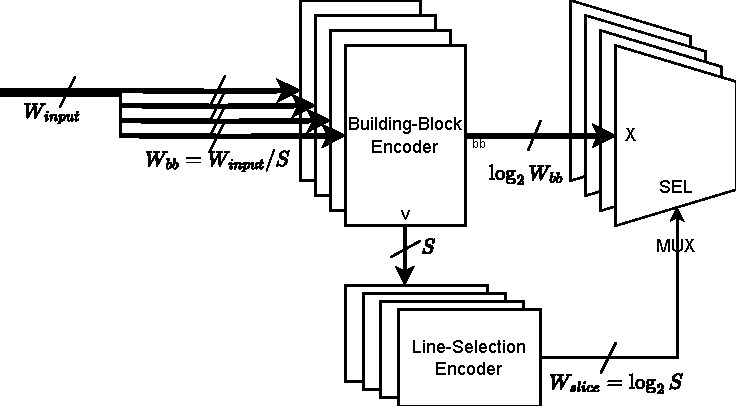
\includegraphics[width=0.40\textwidth]{report_lab3.assets/data_model_crop.pdf}
    \caption{Data flow and time complexity of the internal}
    \label{data_model}
  \end{center}
\end{figure}

It's obvious that the time complexity of the cascaded architecture priority encoder is \(\mathcal{O}(W_{in})\). If the division is only made once, which is equivalent to building block encoder and line selection generator are confined to cascaded architecture, the total delay is therefore obtained:

\begin{eqnarray}
  D&=&\mathcal{O}(W_{bb})+\mathcal{O}(S)=O\left(\frac{W_{input}}{S}+S\right) \\
  \Rightarrow S &=& \mathop{\mathrm{arg}\ \min}_{S}\left(\frac{W_{input}}{S}+S\right)\\
  &=& W_{input}^{\frac{1}{2}}, \\
  D_{\min} &=& 2S = 2W_{input}^{\frac{1}{2}}
\end{eqnarray}

For divide-conquer implementation with large width input bus, the cascaded architecture delay \(S\) itself is unsatisfying, suggesting that the \(N\)-branch tree architecture (\ref{n_branch_tree}) should be applied.

\begin{figure}[htpb]
  \begin{center}
    \subfloat[N-branch tree architecture illustration]{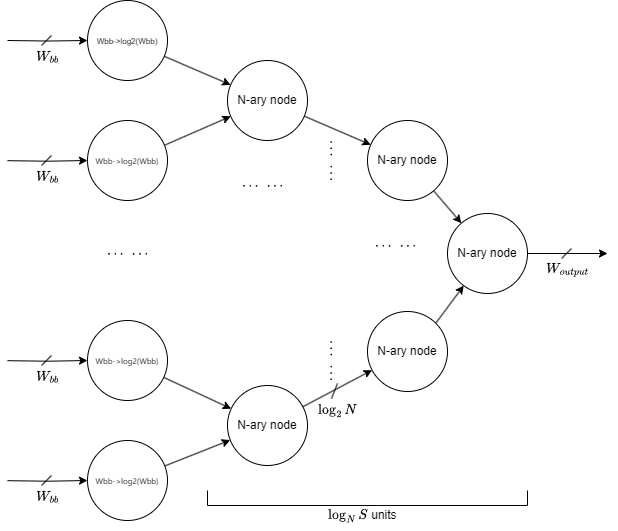
\includegraphics[width=0.40\textwidth]{report_lab3.assets/tree_arch_model.png}}\hspace{0.05\textwidth}
    \subfloat[N-branch tree computational block diagram]{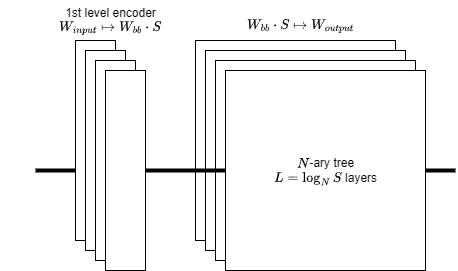
\includegraphics[width=0.40\textwidth]{report_lab3.assets/tree_N_ary_arch_model.png}}
    \caption{N-branch tree architecture}
    \label{n_branch_tree}
  \end{center}
\end{figure}

With the illustration of Fig.(\ref{n_branch_tree} (b)) and respect to the power-2 integrity of \(W, S, N\), take the notion at the output side \(W=2^{w}, S=2^{s}, N=2^{n}\) and then obtain the following time complexity objective:

\begin{eqnarray}
  TC(s,n)&=&\mathcal{O}\left(\frac{W}{S}+L\cdot N\right) \\
  &=&\mathcal{O}\left(2^{w-s}+2^{n}\frac{s}{n}\right)
\end{eqnarray}

Since there is no implied constraints and both \(n\) and \(s\) are positive integers, the extremum can be directly derived by Hessian matrix:

\begin{eqnarray}
  \mathop{\mathrm{arg}\ \min_{(s,n)}}\ TC(s,n) &=& \mathop{\mathrm{arg}}_{(s,n)} \left(\nabla\left(\frac{W}{S}+L\cdot N\right)=0\right) \\
  \Rightarrow (s,n) &=& (w-\log_2 e, \log_2 e)
\end{eqnarray}

and the extremum point satisfies the multiple variable minima condition

\begin{equation}
  \det H|_{(s,n)}=\nabla (TC(i,j)) \nabla^{T} (TC(i,j))|_{(s,n)} > 0
\end{equation}

Applying the integrity constraints to the solution in real domain \((s,n) = (w-\log_2 e, \log_2 e)\), further discussion reveals

\begin{itemize}
  \item For variable \(n\), rounding to \(n=1\) or \(n=2\) results in the same value \(2^{n}/n=2\);
  \item For variable \(s\), take \(2^{n}/n=2\) above results in \(s=w-\lfloor \log_2(\log_2(e))+1 \rfloor = w-1\)
\end{itemize}

Therefore in conclusion,

\begin{equation}
  \mathop{\mathrm{arg}\ \min_{(s,n)}}\ TC(s,n), \{n,s,w\}\subseteq \mathbb{Z^{+}} \Rightarrow
  \begin{cases}
    n\in\{1,2\}\\
    s=w-1
  \end{cases}
\end{equation}

\subsection{After Synthesis Stage Analysis}

Vivado synthesizer optimizes the circuit into LUTs, analog switches and programmable ROMs after the synthesis. For low complexity modules like 4-2 priority encoder (\ref{42enc_alternative}), either the cascaded implementation or the simplified combinational logic (using Carnot Diagram) are synthesized into a couple of LUTs with unit gate delay. For LUT implementation, the submodule is synthesized into an ROM, also with unit gate delay.

\begin{figure}[htpb]
  \begin{center}
    \subfloat[Simplified combinational logic implementation]{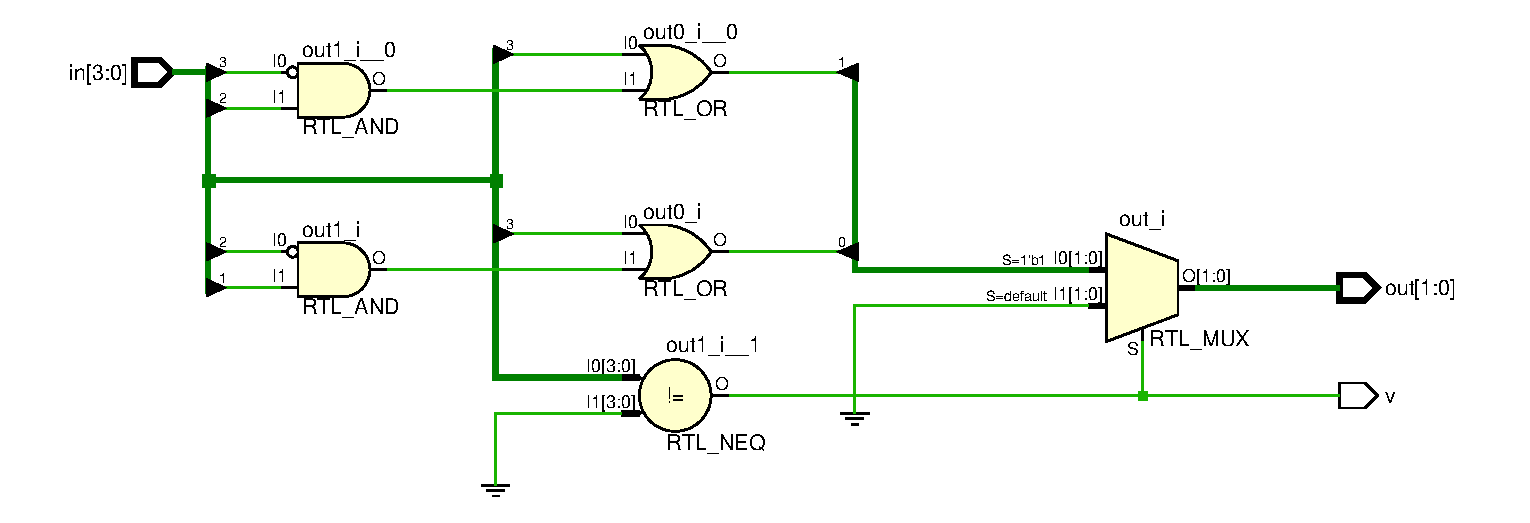
\includegraphics[width=0.42\textwidth]{report_lab3.assets/encoder_elab_1.pdf}}\hspace{0.05\textwidth}
    \subfloat[LUT implementation]{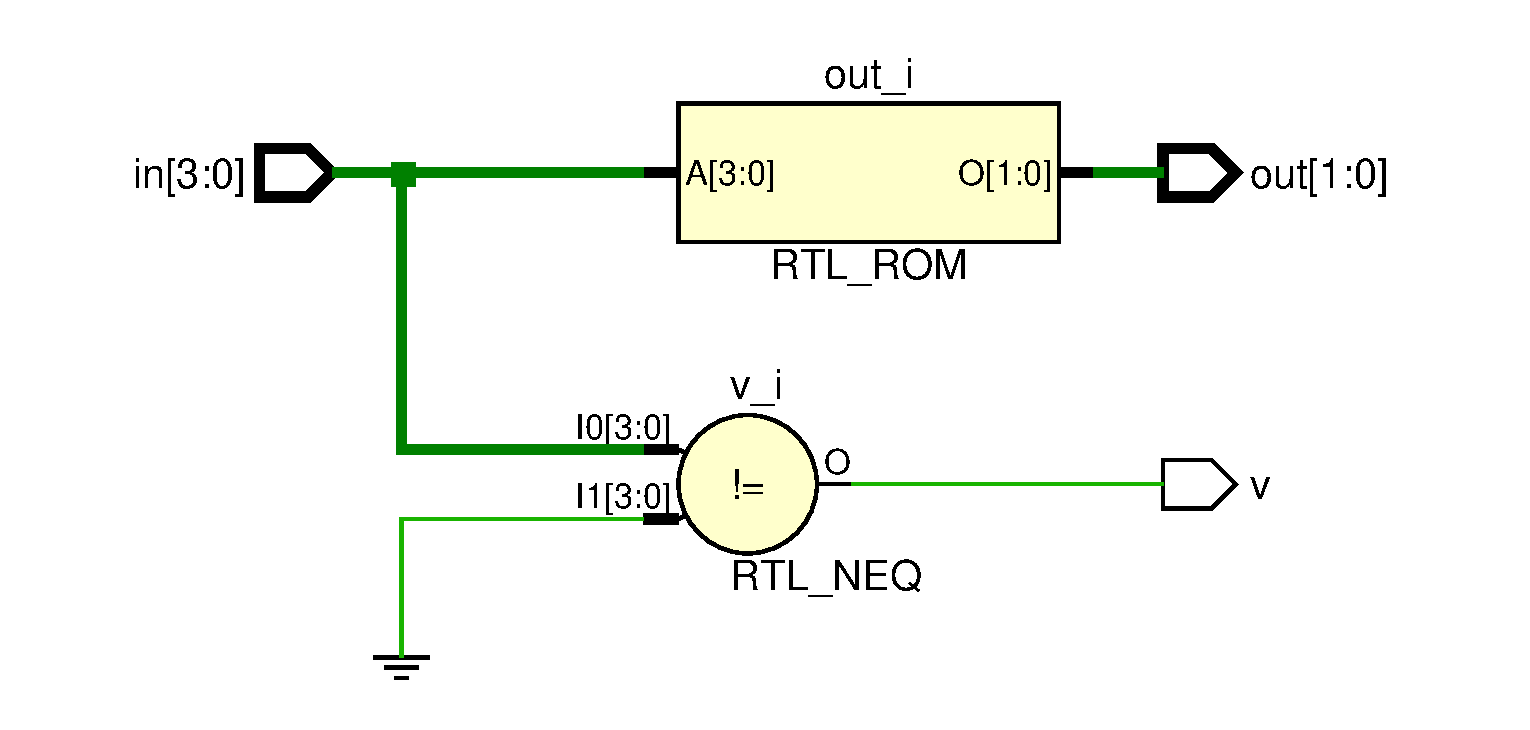
\includegraphics[width=0.42\textwidth]{report_lab3.assets/encoder_LUT_elab_1.pdf}}
    \caption{Alternative implementation of 4-2 encoder submodule}
    \label{42enc_alternative}
  \end{center}
\end{figure}

Thus in the time complexity object Eq.(11), the unit submodule delay suggests that

\begin{equation}
  \frac{W}{S}=1, N=1 \Rightarrow TC(s,n)=\mathcal{O}(L)=\mathcal{O}(\frac{s}{n})
\end{equation}

To minify the possibility of outbounded length in critical paths produced by synthesizer, the input widths \(W_{bb}\) are selected to 4, and the number of layers is \(L=1\). Therefore, parameters selection (6) is still appropriate for the 16-4 priority encoder design.

\section{Simulation Results}

With the elaboration and discussion above, the modeling and simulation are pretty straightforward. Figures below shows the simulation result of 4-2 encoder submodule and the final 16-4 encoder submodule:

\begin{figure}[htpb]
  \begin{center}
    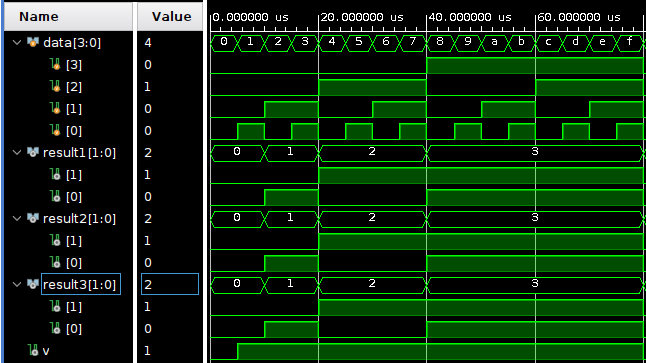
\includegraphics[width=0.6\textwidth]{report_lab3.assets/20240324194920.png}
    \caption{Timing simulation after synthesis of 4-2 priority encoder}
    \label{timing_sim_aftersynth_42}
  \end{center}
\end{figure}

In Fig.(\ref{timing_sim_aftersynth_42}), signal \lstinline{result1} is the output of cascaded architecture submodule, \lstinline{result2} is the output of LUT submodule, and signal \lstinline{result3} is the output of combinational logic (Carnot simplification on design time) submodule.

\begin{figure}[htpb]
  \begin{center}
    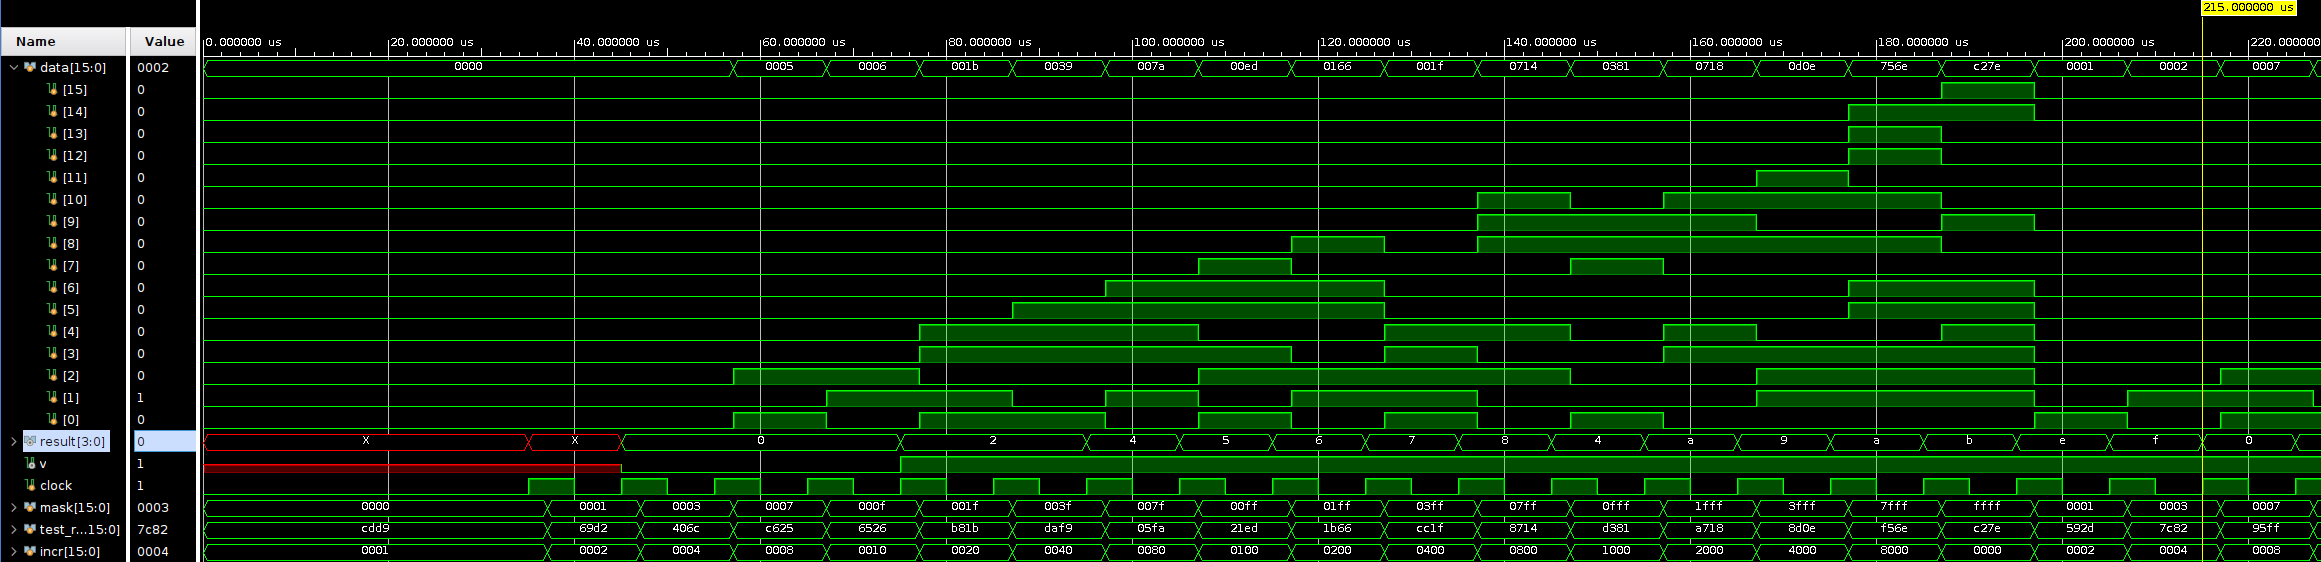
\includegraphics[width=0.95\textwidth]{report_lab3.assets/20240324195347.png}
    \caption{Timing simulation after synthesis of 16-4 priority encoder, using combinational logic submodule}
    \label{timing_sim_aftersynth_164_comb}
  \end{center}
\end{figure}

In Fig.(\ref{timing_sim_aftersynth_164_comb}), the consistency of the 16-4 priority encoder (with 2 layer pipelining) is verified. Note the time required for the initialization of registers at the beginning.

\begin{figure}[htpb]
  \begin{center}
    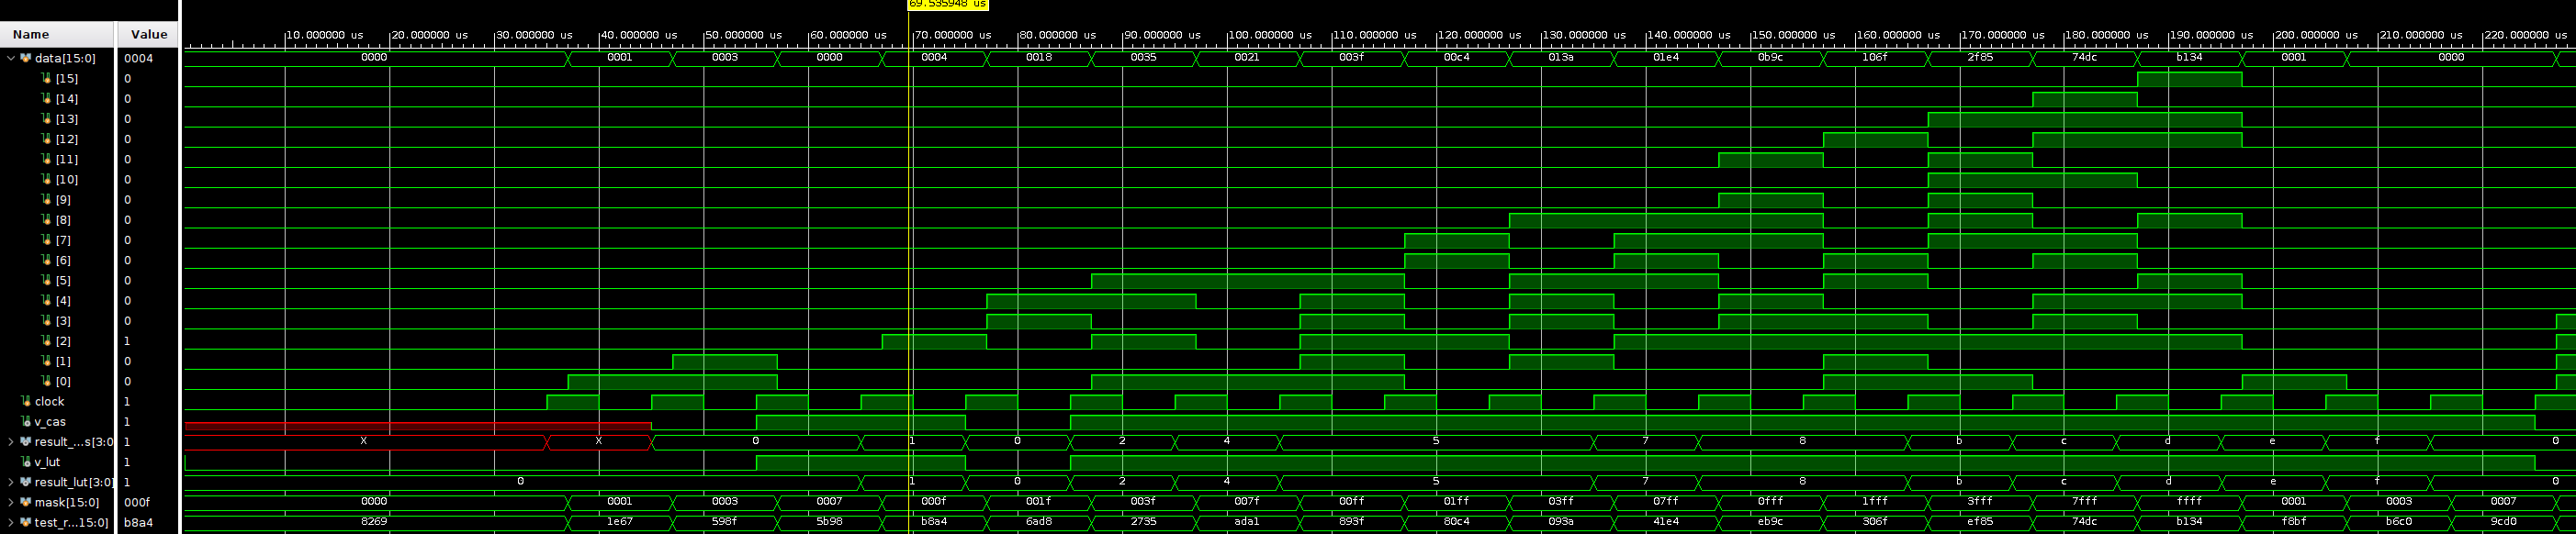
\includegraphics[width=0.95\textwidth]{report_lab3.assets/20240324195739.png}
    \caption{Timing simulation after synthesis of 16-4 priority encoder, using LUT submodule}
    \label{timing_sim_aftersynth_164_lut}
  \end{center}
\end{figure}

In Fig.(\ref{timing_sim_aftersynth_164_lut}), the consistency of the 16-4 priority encoder (with 2 layer pipelining) is verified, the identical critical path between the combinational logic design and the ROM LUT design after synthesis results in identical waveform. Note the time required for the initialization of registers at the beginning.

\section{\textbf{Appendix. Code}}

\subsection{Testbench for 16-4 priority encoder}

\lstinputlisting[language=verilog, style=verilog]{../../../lab3/lab3.srcs/sim_3/new/tb_encoder_16x4_lut.v}

\subsection{Testbench for 4-2 priority encoder}

\lstinputlisting[language=verilog, style=verilog]{../../../lab3/lab3.srcs/sim_1/new/tb_encoder_4to2.v}

\end{document}